\documentclass[1p]{elsarticle_modified}
%\bibliographystyle{elsarticle-num}

%\usepackage[colorlinks]{hyperref}
%\usepackage{abbrmath_seonhwa} %\Abb, \Ascr, \Acal ,\Abf, \Afrak
\usepackage{amsfonts}
\usepackage{amssymb}
\usepackage{amsmath}
\usepackage{amsthm}
\usepackage{scalefnt}
\usepackage{amsbsy}
\usepackage{kotex}
\usepackage{caption}
\usepackage{subfig}
\usepackage{color}
\usepackage{graphicx}
\usepackage{xcolor} %% white, black, red, green, blue, cyan, magenta, yellow
\usepackage{float}
\usepackage{setspace}
\usepackage{hyperref}

\usepackage{tikz}
\usetikzlibrary{arrows}

\usepackage{multirow}
\usepackage{array} % fixed length table
\usepackage{hhline}

%%%%%%%%%%%%%%%%%%%%%
\makeatletter
\renewcommand*\env@matrix[1][\arraystretch]{%
	\edef\arraystretch{#1}%
	\hskip -\arraycolsep
	\let\@ifnextchar\new@ifnextchar
	\array{*\c@MaxMatrixCols c}}
\makeatother %https://tex.stackexchange.com/questions/14071/how-can-i-increase-the-line-spacing-in-a-matrix
%%%%%%%%%%%%%%%

\usepackage[normalem]{ulem}

\newcommand{\msout}[1]{\ifmmode\text{\sout{\ensuremath{#1}}}\else\sout{#1}\fi}
%SOURCE: \msout is \stkout macro in https://tex.stackexchange.com/questions/20609/strikeout-in-math-mode

\newcommand{\cancel}[1]{
	\ifmmode
	{\color{red}\msout{#1}}
	\else
	{\color{red}\sout{#1}}
	\fi
}

\newcommand{\add}[1]{
	{\color{blue}\uwave{#1}}
}

\newcommand{\replace}[2]{
	\ifmmode
	{\color{red}\msout{#1}}{\color{blue}\uwave{#2}}
	\else
	{\color{red}\sout{#1}}{\color{blue}\uwave{#2}}
	\fi
}

\newcommand{\Sol}{\mathcal{S}} %segment
\newcommand{\D}{D} %diagram
\newcommand{\A}{\mathcal{A}} %arc


%%%%%%%%%%%%%%%%%%%%%%%%%%%%%5 test

\def\sl{\operatorname{\textup{SL}}(2,\Cbb)}
\def\psl{\operatorname{\textup{PSL}}(2,\Cbb)}
\def\quan{\mkern 1mu \triangleright \mkern 1mu}

\theoremstyle{definition}
\newtheorem{thm}{Theorem}[section]
\newtheorem{prop}[thm]{Proposition}
\newtheorem{lem}[thm]{Lemma}
\newtheorem{ques}[thm]{Question}
\newtheorem{cor}[thm]{Corollary}
\newtheorem{defn}[thm]{Definition}
\newtheorem{exam}[thm]{Example}
\newtheorem{rmk}[thm]{Remark}
\newtheorem{alg}[thm]{Algorithm}

\newcommand{\I}{\sqrt{-1}}
\begin{document}

%\begin{frontmatter}
%
%\title{Boundary parabolic representations of knots up to 8 crossings}
%
%%% Group authors per affiliation:
%\author{Yunhi Cho} 
%\address{Department of Mathematics, University of Seoul, Seoul, Korea}
%\ead{yhcho@uos.ac.kr}
%
%
%\author{Seonhwa Kim} %\fnref{s_kim}}
%\address{Center for Geometry and Physics, Institute for Basic Science, Pohang, 37673, Korea}
%\ead{ryeona17@ibs.re.kr}
%
%\author{Hyuk Kim}
%\address{Department of Mathematical Sciences, Seoul National University, Seoul 08826, Korea}
%\ead{hyukkim@snu.ac.kr}
%
%\author{Seokbeom Yoon}
%\address{Department of Mathematical Sciences, Seoul National University, Seoul, 08826,  Korea}
%\ead{sbyoon15@snu.ac.kr}
%
%\begin{abstract}
%We find all boundary parabolic representation of knots up to 8 crossings.
%
%\end{abstract}
%\begin{keyword}
%    \MSC[2010] 57M25 
%\end{keyword}
%
%\end{frontmatter}

%\linenumbers
%\tableofcontents
%
\newcommand\colored[1]{\textcolor{white}{\rule[-0.35ex]{0.8em}{1.4ex}}\kern-0.8em\color{red} #1}%
%\newcommand\colored[1]{\textcolor{white}{ #1}\kern-2.17ex	\textcolor{white}{ #1}\kern-1.81ex	\textcolor{white}{ #1}\kern-2.15ex\color{red}#1	}

{\Large $\underline{12n_{0623}~(K12n_{0623})}$}

\setlength{\tabcolsep}{10pt}
\renewcommand{\arraystretch}{1.6}
\vspace{1cm}\begin{tabular}{m{100pt}>{\centering\arraybackslash}m{274pt}}
\multirow{5}{120pt}{
	\centering
	\includegraphics[width=112pt]{../../../GIT/diagram.site/Diagrams/png/2712_12n_0623.png}\\
\ \ \ A knot diagram\footnotemark}&
\allowdisplaybreaks
\textbf{Linearized knot diagam} \\
\cline{2-2}
 &
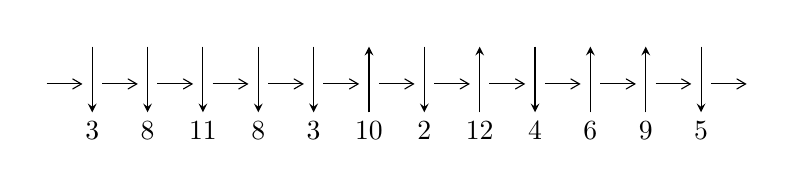
\begin{tikzpicture}[x=20pt, y=17pt]
	% nodes
	\node (C0) at (0, 0) {};
	\node (C1) at (1, 0) {};
	\node (C1U) at (1, +1) {};
	\node (C1D) at (1, -1) {3};

	\node (C2) at (2, 0) {};
	\node (C2U) at (2, +1) {};
	\node (C2D) at (2, -1) {8};

	\node (C3) at (3, 0) {};
	\node (C3U) at (3, +1) {};
	\node (C3D) at (3, -1) {11};

	\node (C4) at (4, 0) {};
	\node (C4U) at (4, +1) {};
	\node (C4D) at (4, -1) {8};

	\node (C5) at (5, 0) {};
	\node (C5U) at (5, +1) {};
	\node (C5D) at (5, -1) {3};

	\node (C6) at (6, 0) {};
	\node (C6U) at (6, +1) {};
	\node (C6D) at (6, -1) {10};

	\node (C7) at (7, 0) {};
	\node (C7U) at (7, +1) {};
	\node (C7D) at (7, -1) {2};

	\node (C8) at (8, 0) {};
	\node (C8U) at (8, +1) {};
	\node (C8D) at (8, -1) {12};

	\node (C9) at (9, 0) {};
	\node (C9U) at (9, +1) {};
	\node (C9D) at (9, -1) {4};

	\node (C10) at (10, 0) {};
	\node (C10U) at (10, +1) {};
	\node (C10D) at (10, -1) {6};

	\node (C11) at (11, 0) {};
	\node (C11U) at (11, +1) {};
	\node (C11D) at (11, -1) {9};

	\node (C12) at (12, 0) {};
	\node (C12U) at (12, +1) {};
	\node (C12D) at (12, -1) {5};
	\node (C13) at (13, 0) {};

	% arrows
	\draw[->,>={angle 60}]
	(C0) edge (C1) (C1) edge (C2) (C2) edge (C3) (C3) edge (C4) (C4) edge (C5) (C5) edge (C6) (C6) edge (C7) (C7) edge (C8) (C8) edge (C9) (C9) edge (C10) (C10) edge (C11) (C11) edge (C12) (C12) edge (C13) ;	\draw[->,>=stealth]
	(C1U) edge (C1D) (C2U) edge (C2D) (C3U) edge (C3D) (C4U) edge (C4D) (C5U) edge (C5D) (C6D) edge (C6U) (C7U) edge (C7D) (C8D) edge (C8U) (C9U) edge (C9D) (C10D) edge (C10U) (C11D) edge (C11U) (C12U) edge (C12D) ;
	\end{tikzpicture} \\
\hhline{~~} \\& 
\textbf{Solving Sequence} \\ \cline{2-2} 
 &
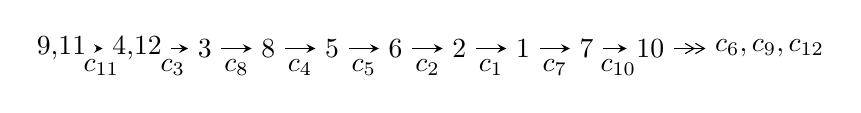
\begin{tikzpicture}[x=23pt, y=7pt]
	% node
	\node (A0) at (-1/8, 0) {9,11};
	\node (A1) at (17/16, 0) {4,12};
	\node (A2) at (17/8, 0) {3};
	\node (A3) at (25/8, 0) {8};
	\node (A4) at (33/8, 0) {5};
	\node (A5) at (41/8, 0) {6};
	\node (A6) at (49/8, 0) {2};
	\node (A7) at (57/8, 0) {1};
	\node (A8) at (65/8, 0) {7};
	\node (A9) at (73/8, 0) {10};
	\node (C1) at (1/2, -1) {$c_{11}$};
	\node (C2) at (13/8, -1) {$c_{3}$};
	\node (C3) at (21/8, -1) {$c_{8}$};
	\node (C4) at (29/8, -1) {$c_{4}$};
	\node (C5) at (37/8, -1) {$c_{5}$};
	\node (C6) at (45/8, -1) {$c_{2}$};
	\node (C7) at (53/8, -1) {$c_{1}$};
	\node (C8) at (61/8, -1) {$c_{7}$};
	\node (C9) at (69/8, -1) {$c_{10}$};
	\node (A10) at (11, 0) {$c_{6},c_{9},c_{12}$};

	% edge
	\draw[->,>=stealth]	
	(A0) edge (A1) (A1) edge (A2) (A2) edge (A3) (A3) edge (A4) (A4) edge (A5) (A5) edge (A6) (A6) edge (A7) (A7) edge (A8) (A8) edge (A9) ;
	\draw[->>,>={angle 60}]	
	(A9) edge (A10);
\end{tikzpicture} \\ 

\end{tabular} \\

\footnotetext{
The image of knot diagram is generated by the software ``\textbf{Draw programme}" developed by Andrew Bartholomew(\url{http://www.layer8.co.uk/maths/draw/index.htm\#Running-draw}), where we modified some parts for our purpose(\url{https://github.com/CATsTAILs/LinksPainter}).
}\phantom \\ \newline 
\centering \textbf{Ideals for irreducible components\footnotemark of $X_{\text{par}}$} 
 
\begin{align*}
I^u_{1}&=\langle 
-2.63058\times10^{46} u^{50}-6.85822\times10^{46} u^{49}+\cdots+1.47546\times10^{47} b-4.38223\times10^{45},\\
\phantom{I^u_{1}}&\phantom{= \langle  }1.43564\times10^{47} u^{50}+2.66794\times10^{47} u^{49}+\cdots+2.95092\times10^{46} a-8.98457\times10^{47},\;u^{51}+2 u^{50}+\cdots-20 u-1\rangle \\
I^u_{2}&=\langle 
734795 u^{24}-937935 u^{23}+\cdots+1479559 b-7004637,\\
\phantom{I^u_{2}}&\phantom{= \langle  }7267713 u^{24}-29159355 u^{23}+\cdots+10356913 a+53569336,\;u^{25}-3 u^{24}+\cdots+13 u-7\rangle \\
\\
\end{align*}
\raggedright * 2 irreducible components of $\dim_{\mathbb{C}}=0$, with total 76 representations.\\
\footnotetext{All coefficients of polynomials are rational numbers. But the coefficients are sometimes approximated in decimal forms when there is not enough margin.}
\newpage
\renewcommand{\arraystretch}{1}
\centering \section*{I. $I^u_{1}= \langle -2.63\times10^{46} u^{50}-6.86\times10^{46} u^{49}+\cdots+1.48\times10^{47} b-4.38\times10^{45},\;1.44\times10^{47} u^{50}+2.67\times10^{47} u^{49}+\cdots+2.95\times10^{46} a-8.98\times10^{47},\;u^{51}+2 u^{50}+\cdots-20 u-1 \rangle$}
\flushleft \textbf{(i) Arc colorings}\\
\begin{tabular}{m{7pt} m{180pt} m{7pt} m{180pt} }
\flushright $a_{9}=$&$\begin{pmatrix}0\\u\end{pmatrix}$ \\
\flushright $a_{11}=$&$\begin{pmatrix}1\\0\end{pmatrix}$ \\
\flushright $a_{4}=$&$\begin{pmatrix}-4.86506 u^{50}-9.04104 u^{49}+\cdots+401.075 u+30.4466\\0.178289 u^{50}+0.464818 u^{49}+\cdots-1.50621 u+0.0297007\end{pmatrix}$ \\
\flushright $a_{12}=$&$\begin{pmatrix}1\\- u^2\end{pmatrix}$ \\
\flushright $a_{3}=$&$\begin{pmatrix}-4.68677 u^{50}-8.57622 u^{49}+\cdots+399.569 u+30.4763\\0.178289 u^{50}+0.464818 u^{49}+\cdots-1.50621 u+0.0297007\end{pmatrix}$ \\
\flushright $a_{8}=$&$\begin{pmatrix}- u\\u^3+u\end{pmatrix}$ \\
\flushright $a_{5}=$&$\begin{pmatrix}-4.04798 u^{50}-7.68387 u^{49}+\cdots+394.709 u+29.9218\\0.435517 u^{50}+0.759418 u^{49}+\cdots+9.58290 u+0.831538\end{pmatrix}$ \\
\flushright $a_{6}=$&$\begin{pmatrix}-0.492075 u^{50}-1.07500 u^{49}+\cdots+8.84678 u+0.791857\\0.448896 u^{50}+0.866909 u^{49}+\cdots-28.7594 u-1.09977\end{pmatrix}$ \\
\flushright $a_{2}=$&$\begin{pmatrix}-5.17498 u^{50}-9.34209 u^{49}+\cdots+407.539 u+31.1016\\0.116517 u^{50}+0.462241 u^{49}+\cdots-13.1991 u-0.806114\end{pmatrix}$ \\
\flushright $a_{1}=$&$\begin{pmatrix}-1.37890 u^{50}-2.73615 u^{49}+\cdots+223.956 u+19.6475\\0.429385 u^{50}+0.695780 u^{49}+\cdots+26.4629 u+1.76995\end{pmatrix}$ \\
\flushright $a_{7}=$&$\begin{pmatrix}-2.47371 u^{50}-3.53471 u^{49}+\cdots+104.745 u+3.16254\\0.523695 u^{50}+1.61796 u^{49}+\cdots-60.5796 u-4.48349\end{pmatrix}$ \\
\flushright $a_{10}=$&$\begin{pmatrix}2.06937 u^{50}+4.75975 u^{49}+\cdots-212.579 u-11.9991\\0.00104699 u^{50}+0.319182 u^{49}+\cdots+22.4132 u+2.24661\end{pmatrix}$\\&\end{tabular}
\flushleft \textbf{(ii) Obstruction class $= -1$}\\~\\
\flushleft \textbf{(iii) Cusp Shapes $= -0.340250 u^{50}+1.20422 u^{49}+\cdots-76.8449 u-18.3790$}\\~\\
\newpage\renewcommand{\arraystretch}{1}
\flushleft \textbf{(iv) u-Polynomials at the component}\newline \\
\begin{tabular}{m{50pt}|m{274pt}}
Crossings & \hspace{64pt}u-Polynomials at each crossing \\
\hline $$\begin{aligned}c_{1}\end{aligned}$$&$\begin{aligned}
&u^{51}+79 u^{50}+\cdots+3170864 u+157609
\end{aligned}$\\
\hline $$\begin{aligned}c_{2},c_{7}\end{aligned}$$&$\begin{aligned}
&u^{51}- u^{50}+\cdots+5960 u-397
\end{aligned}$\\
\hline $$\begin{aligned}c_{3}\end{aligned}$$&$\begin{aligned}
&u^{51}+3 u^{50}+\cdots+1255 u+1525
\end{aligned}$\\
\hline $$\begin{aligned}c_{4}\end{aligned}$$&$\begin{aligned}
&u^{51}+5 u^{50}+\cdots+121755522 u+25773061
\end{aligned}$\\
\hline $$\begin{aligned}c_{5}\end{aligned}$$&$\begin{aligned}
&u^{51}+8 u^{50}+\cdots+281253 u-27881
\end{aligned}$\\
\hline $$\begin{aligned}c_{6},c_{10}\end{aligned}$$&$\begin{aligned}
&u^{51}-2 u^{50}+\cdots+6 u+1
\end{aligned}$\\
\hline $$\begin{aligned}c_{8},c_{11}\end{aligned}$$&$\begin{aligned}
&u^{51}+2 u^{50}+\cdots-20 u-1
\end{aligned}$\\
\hline $$\begin{aligned}c_{9}\end{aligned}$$&$\begin{aligned}
&u^{51}- u^{50}+\cdots+1746 u+2359
\end{aligned}$\\
\hline $$\begin{aligned}c_{12}\end{aligned}$$&$\begin{aligned}
&u^{51}-48 u^{49}+\cdots-2629425 u-635671
\end{aligned}$\\
\hline
\end{tabular}\\~\\
\newpage\renewcommand{\arraystretch}{1}
\flushleft \textbf{(v) Riley Polynomials at the component}\newline \\
\begin{tabular}{m{50pt}|m{274pt}}
Crossings & \hspace{64pt}Riley Polynomials at each crossing \\
\hline $$\begin{aligned}c_{1}\end{aligned}$$&$\begin{aligned}
&y^{51}-199 y^{50}+\cdots-14350346271952 y-24840596881
\end{aligned}$\\
\hline $$\begin{aligned}c_{2},c_{7}\end{aligned}$$&$\begin{aligned}
&y^{51}-79 y^{50}+\cdots+3170864 y-157609
\end{aligned}$\\
\hline $$\begin{aligned}c_{3}\end{aligned}$$&$\begin{aligned}
&y^{51}-25 y^{50}+\cdots-12525125 y-2325625
\end{aligned}$\\
\hline $$\begin{aligned}c_{4}\end{aligned}$$&$\begin{aligned}
&y^{51}-67 y^{50}+\cdots+3374348243821274 y-664250673309721
\end{aligned}$\\
\hline $$\begin{aligned}c_{5}\end{aligned}$$&$\begin{aligned}
&y^{51}-100 y^{50}+\cdots+13844981409 y-777350161
\end{aligned}$\\
\hline $$\begin{aligned}c_{6},c_{10}\end{aligned}$$&$\begin{aligned}
&y^{51}+48 y^{50}+\cdots+156 y-1
\end{aligned}$\\
\hline $$\begin{aligned}c_{8},c_{11}\end{aligned}$$&$\begin{aligned}
&y^{51}+40 y^{50}+\cdots+128 y-1
\end{aligned}$\\
\hline $$\begin{aligned}c_{9}\end{aligned}$$&$\begin{aligned}
&y^{51}-23 y^{50}+\cdots-93576124 y-5564881
\end{aligned}$\\
\hline $$\begin{aligned}c_{12}\end{aligned}$$&$\begin{aligned}
&y^{51}-96 y^{50}+\cdots-3893761828431 y-404077620241
\end{aligned}$\\
\hline
\end{tabular}\\~\\
\newpage\flushleft \textbf{(vi) Complex Volumes and Cusp Shapes}
$$\begin{array}{c|c|c}  
\text{Solutions to }I^u_{1}& \I (\text{vol} + \sqrt{-1}CS) & \text{Cusp shape}\\
 \hline 
\begin{aligned}
u &= -0.994138 + 0.085954 I \\
a &= -1.353360 - 0.114217 I \\
b &= \phantom{-}1.269410 + 0.406751 I\end{aligned}
 & -5.19174 - 2.40432 I & -8.36352 + 1.90027 I \\ \hline\begin{aligned}
u &= -0.994138 - 0.085954 I \\
a &= -1.353360 + 0.114217 I \\
b &= \phantom{-}1.269410 - 0.406751 I\end{aligned}
 & -5.19174 + 2.40432 I & -8.36352 - 1.90027 I \\ \hline\begin{aligned}
u &= \phantom{-}0.786614 + 0.574148 I \\
a &= \phantom{-}0.427916 + 0.361953 I \\
b &= \phantom{-}0.026370 - 0.354661 I\end{aligned}
 & \phantom{-}1.35251 + 1.31026 I & \phantom{-}5.81869 - 2.67401 I \\ \hline\begin{aligned}
u &= \phantom{-}0.786614 - 0.574148 I \\
a &= \phantom{-}0.427916 - 0.361953 I \\
b &= \phantom{-}0.026370 + 0.354661 I\end{aligned}
 & \phantom{-}1.35251 - 1.31026 I & \phantom{-}5.81869 + 2.67401 I \\ \hline\begin{aligned}
u &= -1.106830 + 0.122939 I \\
a &= \phantom{-}1.20913 + 0.99476 I \\
b &= -1.38251 - 0.85821 I\end{aligned}
 & -16.0490 - 8.5925 I & -7.67000 + 4.03651 I \\ \hline\begin{aligned}
u &= -1.106830 - 0.122939 I \\
a &= \phantom{-}1.20913 - 0.99476 I \\
b &= -1.38251 + 0.85821 I\end{aligned}
 & -16.0490 + 8.5925 I & -7.67000 - 4.03651 I \\ \hline\begin{aligned}
u &= \phantom{-}0.852088 + 0.208570 I \\
a &= \phantom{-}0.207993 + 0.892841 I \\
b &= \phantom{-}0.149185 - 0.737393 I\end{aligned}
 & \phantom{-}1.55720 + 1.17905 I & \phantom{-}3.83068 - 5.32777 I \\ \hline\begin{aligned}
u &= \phantom{-}0.852088 - 0.208570 I \\
a &= \phantom{-}0.207993 - 0.892841 I \\
b &= \phantom{-}0.149185 + 0.737393 I\end{aligned}
 & \phantom{-}1.55720 - 1.17905 I & \phantom{-}3.83068 + 5.32777 I \\ \hline\begin{aligned}
u &= \phantom{-}0.026626 + 1.187680 I \\
a &= -0.614290 - 0.648940 I \\
b &= -1.093360 + 0.724987 I\end{aligned}
 & -3.93895 - 0.13627 I & -8.12420 + 0. I\phantom{ +0.000000I} \\ \hline\begin{aligned}
u &= \phantom{-}0.026626 - 1.187680 I \\
a &= -0.614290 + 0.648940 I \\
b &= -1.093360 - 0.724987 I\end{aligned}
 & -3.93895 + 0.13627 I & -8.12420 + 0. I\phantom{ +0.000000I}\\
 \hline 
 \end{array}$$\newpage$$\begin{array}{c|c|c}  
\text{Solutions to }I^u_{1}& \I (\text{vol} + \sqrt{-1}CS) & \text{Cusp shape}\\
 \hline 
\begin{aligned}
u &= \phantom{-}0.310319 + 1.178590 I \\
a &= \phantom{-}0.422592 + 0.832622 I \\
b &= \phantom{-}0.701422 - 0.894046 I\end{aligned}
 & -1.33059 + 2.80047 I & \phantom{-0.000000 } 0 \\ \hline\begin{aligned}
u &= \phantom{-}0.310319 - 1.178590 I \\
a &= \phantom{-}0.422592 - 0.832622 I \\
b &= \phantom{-}0.701422 + 0.894046 I\end{aligned}
 & -1.33059 - 2.80047 I & \phantom{-0.000000 } 0 \\ \hline\begin{aligned}
u &= \phantom{-}0.158146 + 1.210580 I \\
a &= \phantom{-}2.63622 - 0.93189 I \\
b &= \phantom{-}0.669895 - 0.455137 I\end{aligned}
 & -17.1653 + 1.7421 I & \phantom{-0.000000 } 0 \\ \hline\begin{aligned}
u &= \phantom{-}0.158146 - 1.210580 I \\
a &= \phantom{-}2.63622 + 0.93189 I \\
b &= \phantom{-}0.669895 + 0.455137 I\end{aligned}
 & -17.1653 - 1.7421 I & \phantom{-0.000000 } 0 \\ \hline\begin{aligned}
u &= \phantom{-}1.22316\phantom{ +0.000000I} \\
a &= \phantom{-}1.10222\phantom{ +0.000000I} \\
b &= -1.25545\phantom{ +0.000000I}\end{aligned}
 & -10.6865\phantom{ +0.000000I} & -8.45790\phantom{ +0.000000I} \\ \hline\begin{aligned}
u &= -0.288984 + 1.202430 I \\
a &= \phantom{-}0.47810 - 1.51286 I \\
b &= \phantom{-}1.034950 + 0.604820 I\end{aligned}
 & -4.73867 - 6.03590 I & \phantom{-0.000000 } 0 \\ \hline\begin{aligned}
u &= -0.288984 - 1.202430 I \\
a &= \phantom{-}0.47810 + 1.51286 I \\
b &= \phantom{-}1.034950 - 0.604820 I\end{aligned}
 & -4.73867 + 6.03590 I & \phantom{-0.000000 } 0 \\ \hline\begin{aligned}
u &= -0.058157 + 0.755707 I \\
a &= -0.636801 - 0.138149 I \\
b &= \phantom{-}0.020839 + 0.840879 I\end{aligned}
 & -2.04460 - 0.19383 I & -7.78460 + 0.50141 I \\ \hline\begin{aligned}
u &= -0.058157 - 0.755707 I \\
a &= -0.636801 + 0.138149 I \\
b &= \phantom{-}0.020839 - 0.840879 I\end{aligned}
 & -2.04460 + 0.19383 I & -7.78460 - 0.50141 I \\ \hline\begin{aligned}
u &= -0.084630 + 1.245450 I \\
a &= -0.278589 + 0.972468 I \\
b &= -1.54630 - 1.46810 I\end{aligned}
 & -7.13833 - 3.92211 I & \phantom{-0.000000 } 0\\
 \hline 
 \end{array}$$\newpage$$\begin{array}{c|c|c}  
\text{Solutions to }I^u_{1}& \I (\text{vol} + \sqrt{-1}CS) & \text{Cusp shape}\\
 \hline 
\begin{aligned}
u &= -0.084630 - 1.245450 I \\
a &= -0.278589 - 0.972468 I \\
b &= -1.54630 + 1.46810 I\end{aligned}
 & -7.13833 + 3.92211 I & \phantom{-0.000000 } 0 \\ \hline\begin{aligned}
u &= \phantom{-}0.016591 + 1.259310 I \\
a &= -0.702940 + 1.065780 I \\
b &= -0.894998 + 0.074500 I\end{aligned}
 & -7.74070 + 2.61044 I & \phantom{-0.000000 } 0 \\ \hline\begin{aligned}
u &= \phantom{-}0.016591 - 1.259310 I \\
a &= -0.702940 - 1.065780 I \\
b &= -0.894998 - 0.074500 I\end{aligned}
 & -7.74070 - 2.61044 I & \phantom{-0.000000 } 0 \\ \hline\begin{aligned}
u &= -0.220765 + 1.247150 I \\
a &= -0.083136 - 0.648485 I \\
b &= \phantom{-}1.56558 + 0.49642 I\end{aligned}
 & -5.51008 - 0.25342 I & \phantom{-0.000000 } 0 \\ \hline\begin{aligned}
u &= -0.220765 - 1.247150 I \\
a &= -0.083136 + 0.648485 I \\
b &= \phantom{-}1.56558 - 0.49642 I\end{aligned}
 & -5.51008 + 0.25342 I & \phantom{-0.000000 } 0 \\ \hline\begin{aligned}
u &= -0.159806 + 1.260190 I \\
a &= \phantom{-}0.772250 + 0.695570 I \\
b &= \phantom{-}0.721665 - 0.654312 I\end{aligned}
 & -11.89480 - 2.24028 I & \phantom{-0.000000 } 0 \\ \hline\begin{aligned}
u &= -0.159806 - 1.260190 I \\
a &= \phantom{-}0.772250 - 0.695570 I \\
b &= \phantom{-}0.721665 + 0.654312 I\end{aligned}
 & -11.89480 + 2.24028 I & \phantom{-0.000000 } 0 \\ \hline\begin{aligned}
u &= \phantom{-}0.161089 + 1.307720 I \\
a &= -0.387695 - 0.725680 I \\
b &= \phantom{-}1.45529 + 2.33010 I\end{aligned}
 & -18.3648 + 2.7821 I & \phantom{-0.000000 } 0 \\ \hline\begin{aligned}
u &= \phantom{-}0.161089 - 1.307720 I \\
a &= -0.387695 + 0.725680 I \\
b &= \phantom{-}1.45529 - 2.33010 I\end{aligned}
 & -18.3648 - 2.7821 I & \phantom{-0.000000 } 0 \\ \hline\begin{aligned}
u &= \phantom{-}0.689622 + 1.168360 I \\
a &= \phantom{-}0.106520 + 0.152425 I \\
b &= -0.293292 - 0.510638 I\end{aligned}
 & -0.59495 + 4.55029 I & \phantom{-0.000000 } 0\\
 \hline 
 \end{array}$$\newpage$$\begin{array}{c|c|c}  
\text{Solutions to }I^u_{1}& \I (\text{vol} + \sqrt{-1}CS) & \text{Cusp shape}\\
 \hline 
\begin{aligned}
u &= \phantom{-}0.689622 - 1.168360 I \\
a &= \phantom{-}0.106520 - 0.152425 I \\
b &= -0.293292 + 0.510638 I\end{aligned}
 & -0.59495 - 4.55029 I & \phantom{-0.000000 } 0 \\ \hline\begin{aligned}
u &= -0.622814 + 0.099336 I \\
a &= \phantom{-}1.58845 - 0.82975 I \\
b &= -0.913841 + 0.194293 I\end{aligned}
 & -1.42485 + 2.61753 I & -2.41324 - 1.50958 I \\ \hline\begin{aligned}
u &= -0.622814 - 0.099336 I \\
a &= \phantom{-}1.58845 + 0.82975 I \\
b &= -0.913841 - 0.194293 I\end{aligned}
 & -1.42485 - 2.61753 I & -2.41324 + 1.50958 I \\ \hline\begin{aligned}
u &= -0.503411 + 1.302910 I \\
a &= \phantom{-}0.222439 + 1.271540 I \\
b &= -1.185630 - 0.129138 I\end{aligned}
 & -9.00099 - 2.99057 I & \phantom{-0.000000 } 0 \\ \hline\begin{aligned}
u &= -0.503411 - 1.302910 I \\
a &= \phantom{-}0.222439 - 1.271540 I \\
b &= -1.185630 + 0.129138 I\end{aligned}
 & -9.00099 + 2.99057 I & \phantom{-0.000000 } 0 \\ \hline\begin{aligned}
u &= \phantom{-}0.40947 + 1.36366 I \\
a &= -0.526747 - 0.671786 I \\
b &= -0.752311 + 0.792221 I\end{aligned}
 & -3.31584 + 5.81138 I & \phantom{-0.000000 } 0 \\ \hline\begin{aligned}
u &= \phantom{-}0.40947 - 1.36366 I \\
a &= -0.526747 + 0.671786 I \\
b &= -0.752311 - 0.792221 I\end{aligned}
 & -3.31584 - 5.81138 I & \phantom{-0.000000 } 0 \\ \hline\begin{aligned}
u &= -0.42839 + 1.36330 I \\
a &= \phantom{-}0.044190 + 0.982449 I \\
b &= -1.81626 - 0.80792 I\end{aligned}
 & -9.79831 - 7.44096 I & \phantom{-0.000000 } 0 \\ \hline\begin{aligned}
u &= -0.42839 - 1.36330 I \\
a &= \phantom{-}0.044190 - 0.982449 I \\
b &= -1.81626 + 0.80792 I\end{aligned}
 & -9.79831 + 7.44096 I & \phantom{-0.000000 } 0 \\ \hline\begin{aligned}
u &= -0.49015 + 1.41710 I \\
a &= \phantom{-}0.274461 - 1.344710 I \\
b &= \phantom{-}1.60591 + 1.08179 I\end{aligned}
 & \phantom{-}18.5631 - 14.2339 I & \phantom{-0.000000 } 0\\
 \hline 
 \end{array}$$\newpage$$\begin{array}{c|c|c}  
\text{Solutions to }I^u_{1}& \I (\text{vol} + \sqrt{-1}CS) & \text{Cusp shape}\\
 \hline 
\begin{aligned}
u &= -0.49015 - 1.41710 I \\
a &= \phantom{-}0.274461 + 1.344710 I \\
b &= \phantom{-}1.60591 - 1.08179 I\end{aligned}
 & \phantom{-}18.5631 + 14.2339 I & \phantom{-0.000000 } 0 \\ \hline\begin{aligned}
u &= -0.64736 + 1.35681 I \\
a &= -0.744754 - 0.575553 I \\
b &= \phantom{-}1.33716 - 0.48247 I\end{aligned}
 & \phantom{-}19.7044 + 2.3380 I & \phantom{-0.000000 } 0 \\ \hline\begin{aligned}
u &= -0.64736 - 1.35681 I \\
a &= -0.744754 + 0.575553 I \\
b &= \phantom{-}1.33716 + 0.48247 I\end{aligned}
 & \phantom{-}19.7044 - 2.3380 I & \phantom{-0.000000 } 0 \\ \hline\begin{aligned}
u &= \phantom{-}0.473371 + 0.113783 I \\
a &= -1.30948 + 3.62099 I \\
b &= -0.86213 - 1.28518 I\end{aligned}
 & -13.90700 + 0.51978 I & -6.17475 - 0.20171 I \\ \hline\begin{aligned}
u &= \phantom{-}0.473371 - 0.113783 I \\
a &= -1.30948 - 3.62099 I \\
b &= -0.86213 + 1.28518 I\end{aligned}
 & -13.90700 - 0.51978 I & -6.17475 + 0.20171 I \\ \hline\begin{aligned}
u &= -0.466662\phantom{ +0.000000I} \\
a &= -1.70449\phantom{ +0.000000I} \\
b &= -0.595548\phantom{ +0.000000I}\end{aligned}
 & -8.02552\phantom{ +0.000000I} & -22.3740\phantom{ +0.000000I} \\ \hline\begin{aligned}
u &= \phantom{-}0.56332 + 1.45126 I \\
a &= -0.174961 + 0.929296 I \\
b &= \phantom{-}1.39706 - 0.38413 I\end{aligned}
 & -15.3202 + 6.3714 I & \phantom{-0.000000 } 0 \\ \hline\begin{aligned}
u &= \phantom{-}0.56332 - 1.45126 I \\
a &= -0.174961 - 0.929296 I \\
b &= \phantom{-}1.39706 + 0.38413 I\end{aligned}
 & -15.3202 - 6.3714 I & \phantom{-0.000000 } 0 \\ \hline\begin{aligned}
u &= -0.166908 + 0.082981 I \\
a &= -5.15701 - 2.31484 I \\
b &= \phantom{-}0.960493 - 0.750766 I\end{aligned}
 & -3.58169 + 2.87292 I & -8.22764 - 2.63355 I \\ \hline\begin{aligned}
u &= -0.166908 - 0.082981 I \\
a &= -5.15701 + 2.31484 I \\
b &= \phantom{-}0.960493 + 0.750766 I\end{aligned}
 & -3.58169 - 2.87292 I & -8.22764 + 2.63355 I\\
 \hline 
 \end{array}$$\newpage$$\begin{array}{c|c|c}  
\text{Solutions to }I^u_{1}& \I (\text{vol} + \sqrt{-1}CS) & \text{Cusp shape}\\
 \hline 
\begin{aligned}
u &= -0.106308\phantom{ +0.000000I} \\
a &= \phantom{-}3.76128\phantom{ +0.000000I} \\
b &= \phantom{-}0.501782\phantom{ +0.000000I}\end{aligned}
 & -0.859424\phantom{ +0.000000I} & -11.7400\phantom{ +0.000000I}\\
 \hline 
 \end{array}$$\newpage\newpage\renewcommand{\arraystretch}{1}
\centering \section*{II. $I^u_{2}= \langle 7.35\times10^{5} u^{24}-9.38\times10^{5} u^{23}+\cdots+1.48\times10^{6} b-7.00\times10^{6},\;7.27\times10^{6} u^{24}-2.92\times10^{7} u^{23}+\cdots+1.04\times10^{7} a+5.36\times10^{7},\;u^{25}-3 u^{24}+\cdots+13 u-7 \rangle$}
\flushleft \textbf{(i) Arc colorings}\\
\begin{tabular}{m{7pt} m{180pt} m{7pt} m{180pt} }
\flushright $a_{9}=$&$\begin{pmatrix}0\\u\end{pmatrix}$ \\
\flushright $a_{11}=$&$\begin{pmatrix}1\\0\end{pmatrix}$ \\
\flushright $a_{4}=$&$\begin{pmatrix}-0.701726 u^{24}+2.81545 u^{23}+\cdots+11.8091 u-5.17233\\-0.496631 u^{24}+0.633929 u^{23}+\cdots-9.36066 u+4.73427\end{pmatrix}$ \\
\flushright $a_{12}=$&$\begin{pmatrix}1\\- u^2\end{pmatrix}$ \\
\flushright $a_{3}=$&$\begin{pmatrix}-1.19836 u^{24}+3.44938 u^{23}+\cdots+2.44847 u-0.438053\\-0.496631 u^{24}+0.633929 u^{23}+\cdots-9.36066 u+4.73427\end{pmatrix}$ \\
\flushright $a_{8}=$&$\begin{pmatrix}- u\\u^3+u\end{pmatrix}$ \\
\flushright $a_{5}=$&$\begin{pmatrix}-1.87701 u^{24}+5.33929 u^{23}+\cdots+1.97688 u+3.82771\\-1.10959 u^{24}+2.60918 u^{23}+\cdots-4.32774 u+2.74843\end{pmatrix}$ \\
\flushright $a_{6}=$&$\begin{pmatrix}1.10695 u^{24}-3.28329 u^{23}+\cdots-3.85869 u+2.45136\\0.349387 u^{24}-0.152774 u^{23}+\cdots+12.4684 u-7.59653\end{pmatrix}$ \\
\flushright $a_{2}=$&$\begin{pmatrix}-0.677384 u^{24}+2.96821 u^{23}+\cdots+16.9113 u-10.2873\\0.373689 u^{24}-1.86668 u^{23}+\cdots-13.4076 u+7.01127\end{pmatrix}$ \\
\flushright $a_{1}=$&$\begin{pmatrix}3.51385 u^{24}-9.56743 u^{23}+\cdots+5.52009 u-11.3721\\0.870320 u^{24}-1.50061 u^{23}+\cdots+8.95310 u-3.72301\end{pmatrix}$ \\
\flushright $a_{7}=$&$\begin{pmatrix}-1.24978 u^{24}+4.85892 u^{23}+\cdots+15.5740 u+1.08065\\-0.427846 u^{24}+0.336245 u^{23}+\cdots-11.0557 u+5.37195\end{pmatrix}$ \\
\flushright $a_{10}=$&$\begin{pmatrix}-1.53579 u^{24}+2.59613 u^{23}+\cdots-23.5205 u+13.1392\\0.791862 u^{24}-2.31714 u^{23}+\cdots-1.63424 u-0.947584\end{pmatrix}$\\&\end{tabular}
\flushleft \textbf{(ii) Obstruction class $= 1$}\\~\\
\flushleft \textbf{(iii) Cusp Shapes $= \frac{1222669}{1479559} u^{24}-\frac{2760822}{1479559} u^{23}+\cdots-\frac{13385950}{1479559} u+\frac{10657151}{1479559}$}\\~\\
\newpage\renewcommand{\arraystretch}{1}
\flushleft \textbf{(iv) u-Polynomials at the component}\newline \\
\begin{tabular}{m{50pt}|m{274pt}}
Crossings & \hspace{64pt}u-Polynomials at each crossing \\
\hline $$\begin{aligned}c_{1}\end{aligned}$$&$\begin{aligned}
&u^{25}-28 u^{24}+\cdots+97 u-9
\end{aligned}$\\
\hline $$\begin{aligned}c_{2}\end{aligned}$$&$\begin{aligned}
&u^{25}-14 u^{23}+\cdots+5 u+3
\end{aligned}$\\
\hline $$\begin{aligned}c_{3}\end{aligned}$$&$\begin{aligned}
&u^{25}-2 u^{24}+\cdots+2 u-1
\end{aligned}$\\
\hline $$\begin{aligned}c_{4}\end{aligned}$$&$\begin{aligned}
&u^{25}-6 u^{23}+\cdots-3 u+1
\end{aligned}$\\
\hline $$\begin{aligned}c_{5}\end{aligned}$$&$\begin{aligned}
&u^{25}+21 u^{24}+\cdots+2014 u+271
\end{aligned}$\\
\hline $$\begin{aligned}c_{6}\end{aligned}$$&$\begin{aligned}
&u^{25}- u^{24}+\cdots+u-1
\end{aligned}$\\
\hline $$\begin{aligned}c_{7}\end{aligned}$$&$\begin{aligned}
&u^{25}-14 u^{23}+\cdots+5 u-3
\end{aligned}$\\
\hline $$\begin{aligned}c_{8}\end{aligned}$$&$\begin{aligned}
&u^{25}+3 u^{24}+\cdots+13 u+7
\end{aligned}$\\
\hline $$\begin{aligned}c_{9}\end{aligned}$$&$\begin{aligned}
&u^{25}+2 u^{23}+\cdots+11 u-3
\end{aligned}$\\
\hline $$\begin{aligned}c_{10}\end{aligned}$$&$\begin{aligned}
&u^{25}+u^{24}+\cdots+u+1
\end{aligned}$\\
\hline $$\begin{aligned}c_{11}\end{aligned}$$&$\begin{aligned}
&u^{25}-3 u^{24}+\cdots+13 u-7
\end{aligned}$\\
\hline $$\begin{aligned}c_{12}\end{aligned}$$&$\begin{aligned}
&u^{25}+3 u^{24}+\cdots-6 u+1
\end{aligned}$\\
\hline
\end{tabular}\\~\\
\newpage\renewcommand{\arraystretch}{1}
\flushleft \textbf{(v) Riley Polynomials at the component}\newline \\
\begin{tabular}{m{50pt}|m{274pt}}
Crossings & \hspace{64pt}Riley Polynomials at each crossing \\
\hline $$\begin{aligned}c_{1}\end{aligned}$$&$\begin{aligned}
&y^{25}-48 y^{24}+\cdots-3731 y-81
\end{aligned}$\\
\hline $$\begin{aligned}c_{2},c_{7}\end{aligned}$$&$\begin{aligned}
&y^{25}-28 y^{24}+\cdots+97 y-9
\end{aligned}$\\
\hline $$\begin{aligned}c_{3}\end{aligned}$$&$\begin{aligned}
&y^{25}-2 y^{24}+\cdots+20 y-1
\end{aligned}$\\
\hline $$\begin{aligned}c_{4}\end{aligned}$$&$\begin{aligned}
&y^{25}-12 y^{24}+\cdots-9 y-1
\end{aligned}$\\
\hline $$\begin{aligned}c_{5}\end{aligned}$$&$\begin{aligned}
&y^{25}-33 y^{24}+\cdots+697422 y-73441
\end{aligned}$\\
\hline $$\begin{aligned}c_{6},c_{10}\end{aligned}$$&$\begin{aligned}
&y^{25}+15 y^{24}+\cdots-15 y-1
\end{aligned}$\\
\hline $$\begin{aligned}c_{8},c_{11}\end{aligned}$$&$\begin{aligned}
&y^{25}+19 y^{24}+\cdots+29 y-49
\end{aligned}$\\
\hline $$\begin{aligned}c_{9}\end{aligned}$$&$\begin{aligned}
&y^{25}+4 y^{24}+\cdots+73 y-9
\end{aligned}$\\
\hline $$\begin{aligned}c_{12}\end{aligned}$$&$\begin{aligned}
&y^{25}-17 y^{24}+\cdots-10 y-1
\end{aligned}$\\
\hline
\end{tabular}\\~\\
\newpage\flushleft \textbf{(vi) Complex Volumes and Cusp Shapes}
$$\begin{array}{c|c|c}  
\text{Solutions to }I^u_{2}& \I (\text{vol} + \sqrt{-1}CS) & \text{Cusp shape}\\
 \hline 
\begin{aligned}
u &= -0.165879 + 1.036770 I \\
a &= \phantom{-}1.99622 - 0.01072 I \\
b &= \phantom{-}0.178538 - 1.088440 I\end{aligned}
 & -16.3073 - 0.6846 I & -10.58791 - 0.36694 I \\ \hline\begin{aligned}
u &= -0.165879 - 1.036770 I \\
a &= \phantom{-}1.99622 + 0.01072 I \\
b &= \phantom{-}0.178538 + 1.088440 I\end{aligned}
 & -16.3073 + 0.6846 I & -10.58791 + 0.36694 I \\ \hline\begin{aligned}
u &= \phantom{-}0.878653 + 0.614276 I \\
a &= -0.388165 - 0.018797 I \\
b &= \phantom{-}0.519314 - 0.020674 I\end{aligned}
 & \phantom{-}0.87332 + 1.24381 I & -11.80207 - 0.23731 I \\ \hline\begin{aligned}
u &= \phantom{-}0.878653 - 0.614276 I \\
a &= -0.388165 + 0.018797 I \\
b &= \phantom{-}0.519314 + 0.020674 I\end{aligned}
 & \phantom{-}0.87332 - 1.24381 I & -11.80207 + 0.23731 I \\ \hline\begin{aligned}
u &= -0.241992 + 1.085870 I \\
a &= -0.080016 - 1.368120 I \\
b &= \phantom{-}0.99835 + 1.05321 I\end{aligned}
 & -5.21178 - 4.26834 I & -9.53069 + 3.29154 I \\ \hline\begin{aligned}
u &= -0.241992 - 1.085870 I \\
a &= -0.080016 + 1.368120 I \\
b &= \phantom{-}0.99835 - 1.05321 I\end{aligned}
 & -5.21178 + 4.26834 I & -9.53069 - 3.29154 I \\ \hline\begin{aligned}
u &= -0.525469 + 0.701017 I \\
a &= \phantom{-}1.028560 + 0.820742 I \\
b &= -0.762718 + 0.513757 I\end{aligned}
 & -4.05799 + 1.29515 I & -9.79398 + 0.20407 I \\ \hline\begin{aligned}
u &= -0.525469 - 0.701017 I \\
a &= \phantom{-}1.028560 - 0.820742 I \\
b &= -0.762718 - 0.513757 I\end{aligned}
 & -4.05799 - 1.29515 I & -9.79398 - 0.20407 I \\ \hline\begin{aligned}
u &= \phantom{-}0.777677 + 0.135052 I \\
a &= \phantom{-}0.311592 + 1.346060 I \\
b &= \phantom{-}0.258764 - 1.085200 I\end{aligned}
 & \phantom{-}0.620768 + 1.112620 I & -6.49974 - 2.44499 I \\ \hline\begin{aligned}
u &= \phantom{-}0.777677 - 0.135052 I \\
a &= \phantom{-}0.311592 - 1.346060 I \\
b &= \phantom{-}0.258764 + 1.085200 I\end{aligned}
 & \phantom{-}0.620768 - 1.112620 I & -6.49974 + 2.44499 I\\
 \hline 
 \end{array}$$\newpage$$\begin{array}{c|c|c}  
\text{Solutions to }I^u_{2}& \I (\text{vol} + \sqrt{-1}CS) & \text{Cusp shape}\\
 \hline 
\begin{aligned}
u &= \phantom{-}0.310226 + 1.219750 I \\
a &= \phantom{-}0.473117 + 0.758104 I \\
b &= \phantom{-}0.347343 - 1.317550 I\end{aligned}
 & -2.69003 + 2.74082 I & -10.35889 - 2.75940 I \\ \hline\begin{aligned}
u &= \phantom{-}0.310226 - 1.219750 I \\
a &= \phantom{-}0.473117 - 0.758104 I \\
b &= \phantom{-}0.347343 + 1.317550 I\end{aligned}
 & -2.69003 - 2.74082 I & -10.35889 + 2.75940 I \\ \hline\begin{aligned}
u &= -0.080358 + 1.265810 I \\
a &= -0.337318 + 0.390448 I \\
b &= -1.46431 + 0.22680 I\end{aligned}
 & -6.46312 + 1.42279 I & -11.59416 - 0.83507 I \\ \hline\begin{aligned}
u &= -0.080358 - 1.265810 I \\
a &= -0.337318 - 0.390448 I \\
b &= -1.46431 - 0.22680 I\end{aligned}
 & -6.46312 - 1.42279 I & -11.59416 + 0.83507 I \\ \hline\begin{aligned}
u &= -0.688617 + 0.067271 I \\
a &= -1.045060 + 0.756974 I \\
b &= \phantom{-}1.051830 - 0.523343 I\end{aligned}
 & -2.21685 + 3.76261 I & -5.20350 - 5.51009 I \\ \hline\begin{aligned}
u &= -0.688617 - 0.067271 I \\
a &= -1.045060 - 0.756974 I \\
b &= \phantom{-}1.051830 + 0.523343 I\end{aligned}
 & -2.21685 - 3.76261 I & -5.20350 + 5.51009 I \\ \hline\begin{aligned}
u &= -0.357165 + 1.267210 I \\
a &= -0.555297 + 1.045050 I \\
b &= -1.27741 - 0.62995 I\end{aligned}
 & -5.96754 - 7.70508 I & -10.28604 + 7.69329 I \\ \hline\begin{aligned}
u &= -0.357165 - 1.267210 I \\
a &= -0.555297 - 1.045050 I \\
b &= -1.27741 + 0.62995 I\end{aligned}
 & -5.96754 + 7.70508 I & -10.28604 - 7.69329 I \\ \hline\begin{aligned}
u &= \phantom{-}0.159087 + 1.319010 I \\
a &= \phantom{-}0.607715 - 0.734484 I \\
b &= \phantom{-}0.665222 + 0.443905 I\end{aligned}
 & -12.13970 + 2.72655 I & -15.2074 - 7.6255 I \\ \hline\begin{aligned}
u &= \phantom{-}0.159087 - 1.319010 I \\
a &= \phantom{-}0.607715 + 0.734484 I \\
b &= \phantom{-}0.665222 - 0.443905 I\end{aligned}
 & -12.13970 - 2.72655 I & -15.2074 + 7.6255 I\\
 \hline 
 \end{array}$$\newpage$$\begin{array}{c|c|c}  
\text{Solutions to }I^u_{2}& \I (\text{vol} + \sqrt{-1}CS) & \text{Cusp shape}\\
 \hline 
\begin{aligned}
u &= \phantom{-}0.629591\phantom{ +0.000000I} \\
a &= -1.11654\phantom{ +0.000000I} \\
b &= -0.430836\phantom{ +0.000000I}\end{aligned}
 & -7.69986\phantom{ +0.000000I} & \phantom{-}2.83470\phantom{ +0.000000I} \\ \hline\begin{aligned}
u &= \phantom{-}0.367086 + 1.360610 I \\
a &= -0.793602 - 0.650211 I \\
b &= -0.772849 + 0.983417 I\end{aligned}
 & -4.11796 + 5.31027 I & -12.29936 - 3.61405 I \\ \hline\begin{aligned}
u &= \phantom{-}0.367086 - 1.360610 I \\
a &= -0.793602 + 0.650211 I \\
b &= -0.772849 - 0.983417 I\end{aligned}
 & -4.11796 - 5.31027 I & -12.29936 + 3.61405 I \\ \hline\begin{aligned}
u &= \phantom{-}0.75195 + 1.19779 I \\
a &= \phantom{-}0.054806 - 0.462184 I \\
b &= -0.526659 + 0.040712 I\end{aligned}
 & -0.97942 + 4.93110 I & -10.7537 - 10.6108 I \\ \hline\begin{aligned}
u &= \phantom{-}0.75195 - 1.19779 I \\
a &= \phantom{-}0.054806 + 0.462184 I \\
b &= -0.526659 - 0.040712 I\end{aligned}
 & -0.97942 - 4.93110 I & -10.7537 + 10.6108 I\\
 \hline 
 \end{array}$$\newpage
\newpage\renewcommand{\arraystretch}{1}
\centering \section*{ III. u-Polynomials}
\begin{tabular}{m{50pt}|m{274pt}}
Crossings & \hspace{64pt}u-Polynomials at each crossing \\
\hline $$\begin{aligned}c_{1}\end{aligned}$$&$\begin{aligned}
&(u^{25}-28 u^{24}+\cdots+97 u-9)\\
&\cdot(u^{51}+79 u^{50}+\cdots+3170864 u+157609)
\end{aligned}$\\
\hline $$\begin{aligned}c_{2}\end{aligned}$$&$\begin{aligned}
&(u^{25}-14 u^{23}+\cdots+5 u+3)(u^{51}- u^{50}+\cdots+5960 u-397)
\end{aligned}$\\
\hline $$\begin{aligned}c_{3}\end{aligned}$$&$\begin{aligned}
&(u^{25}-2 u^{24}+\cdots+2 u-1)(u^{51}+3 u^{50}+\cdots+1255 u+1525)
\end{aligned}$\\
\hline $$\begin{aligned}c_{4}\end{aligned}$$&$\begin{aligned}
&(u^{25}-6 u^{23}+\cdots-3 u+1)\\
&\cdot(u^{51}+5 u^{50}+\cdots+121755522 u+25773061)
\end{aligned}$\\
\hline $$\begin{aligned}c_{5}\end{aligned}$$&$\begin{aligned}
&(u^{25}+21 u^{24}+\cdots+2014 u+271)\\
&\cdot(u^{51}+8 u^{50}+\cdots+281253 u-27881)
\end{aligned}$\\
\hline $$\begin{aligned}c_{6}\end{aligned}$$&$\begin{aligned}
&(u^{25}- u^{24}+\cdots+u-1)(u^{51}-2 u^{50}+\cdots+6 u+1)
\end{aligned}$\\
\hline $$\begin{aligned}c_{7}\end{aligned}$$&$\begin{aligned}
&(u^{25}-14 u^{23}+\cdots+5 u-3)(u^{51}- u^{50}+\cdots+5960 u-397)
\end{aligned}$\\
\hline $$\begin{aligned}c_{8}\end{aligned}$$&$\begin{aligned}
&(u^{25}+3 u^{24}+\cdots+13 u+7)(u^{51}+2 u^{50}+\cdots-20 u-1)
\end{aligned}$\\
\hline $$\begin{aligned}c_{9}\end{aligned}$$&$\begin{aligned}
&(u^{25}+2 u^{23}+\cdots+11 u-3)(u^{51}- u^{50}+\cdots+1746 u+2359)
\end{aligned}$\\
\hline $$\begin{aligned}c_{10}\end{aligned}$$&$\begin{aligned}
&(u^{25}+u^{24}+\cdots+u+1)(u^{51}-2 u^{50}+\cdots+6 u+1)
\end{aligned}$\\
\hline $$\begin{aligned}c_{11}\end{aligned}$$&$\begin{aligned}
&(u^{25}-3 u^{24}+\cdots+13 u-7)(u^{51}+2 u^{50}+\cdots-20 u-1)
\end{aligned}$\\
\hline $$\begin{aligned}c_{12}\end{aligned}$$&$\begin{aligned}
&(u^{25}+3 u^{24}+\cdots-6 u+1)(u^{51}-48 u^{49}+\cdots-2629425 u-635671)
\end{aligned}$\\
\hline
\end{tabular}\newpage\renewcommand{\arraystretch}{1}
\centering \section*{ IV. Riley Polynomials}
\begin{tabular}{m{50pt}|m{274pt}}
Crossings & \hspace{64pt}Riley Polynomials at each crossing \\
\hline $$\begin{aligned}c_{1}\end{aligned}$$&$\begin{aligned}
&(y^{25}-48 y^{24}+\cdots-3731 y-81)\\
&\cdot(y^{51}-199 y^{50}+\cdots-14350346271952 y-24840596881)
\end{aligned}$\\
\hline $$\begin{aligned}c_{2},c_{7}\end{aligned}$$&$\begin{aligned}
&(y^{25}-28 y^{24}+\cdots+97 y-9)\\
&\cdot(y^{51}-79 y^{50}+\cdots+3170864 y-157609)
\end{aligned}$\\
\hline $$\begin{aligned}c_{3}\end{aligned}$$&$\begin{aligned}
&(y^{25}-2 y^{24}+\cdots+20 y-1)\\
&\cdot(y^{51}-25 y^{50}+\cdots-12525125 y-2325625)
\end{aligned}$\\
\hline $$\begin{aligned}c_{4}\end{aligned}$$&$\begin{aligned}
&(y^{25}-12 y^{24}+\cdots-9 y-1)\\
&\cdot(y^{51}-67 y^{50}+\cdots+3374348243821274 y-664250673309721)
\end{aligned}$\\
\hline $$\begin{aligned}c_{5}\end{aligned}$$&$\begin{aligned}
&(y^{25}-33 y^{24}+\cdots+697422 y-73441)\\
&\cdot(y^{51}-100 y^{50}+\cdots+13844981409 y-777350161)
\end{aligned}$\\
\hline $$\begin{aligned}c_{6},c_{10}\end{aligned}$$&$\begin{aligned}
&(y^{25}+15 y^{24}+\cdots-15 y-1)(y^{51}+48 y^{50}+\cdots+156 y-1)
\end{aligned}$\\
\hline $$\begin{aligned}c_{8},c_{11}\end{aligned}$$&$\begin{aligned}
&(y^{25}+19 y^{24}+\cdots+29 y-49)(y^{51}+40 y^{50}+\cdots+128 y-1)
\end{aligned}$\\
\hline $$\begin{aligned}c_{9}\end{aligned}$$&$\begin{aligned}
&(y^{25}+4 y^{24}+\cdots+73 y-9)\\
&\cdot(y^{51}-23 y^{50}+\cdots-93576124 y-5564881)
\end{aligned}$\\
\hline $$\begin{aligned}c_{12}\end{aligned}$$&$\begin{aligned}
&(y^{25}-17 y^{24}+\cdots-10 y-1)\\
&\cdot(y^{51}-96 y^{50}+\cdots-3893761828431 y-404077620241)
\end{aligned}$\\
\hline
\end{tabular}
\vskip 2pc
\end{document}